\section{Resultados}\label{sec:km_resultados}

\subsection{O efeito do one-hot na distância}\label{sec:cl_onehot}

O K-means agrupa pela distância euclidiana ao quadrado, que soma as diferenças coluna a coluna, de modo que o pré-processamento define o que é ``parecido''. Um atributo numérico padronizado contribui com o quadrado da diferença em desvios; um atributo de texto contribui com 0 quando duas pessoas têm a mesma categoria e com 2 quando têm categorias diferentes, porque uma coluna do one-hot apaga e outra acende, seja qual for o número de categorias. Assim, trocar de ocupação afasta duas pessoas tanto quanto \clTrocaAnos{} anos de diferença de idade ($\sqrt{2}$ desvios de \clDesvioIdade{} anos). Em média, porém, os atributos de texto pesam menos que os numéricos (Figura~\ref{fig:cl_peso}): para duas pessoas sorteadas, cada numérico contribui com 2, e cada atributo de texto com 2 vezes a chance de as duas terem categorias diferentes. Os 5 de texto respondem por \clParteTexto\% da distância média; o país, só por \clPartePais\%, porque 91\% das pessoas são dos EUA. A média esconde a forma: os numéricos variam aos poucos, e as categorias são degraus que tendem a marcar as fronteiras entre os grupos.

\begin{figure}[ht]
\centering
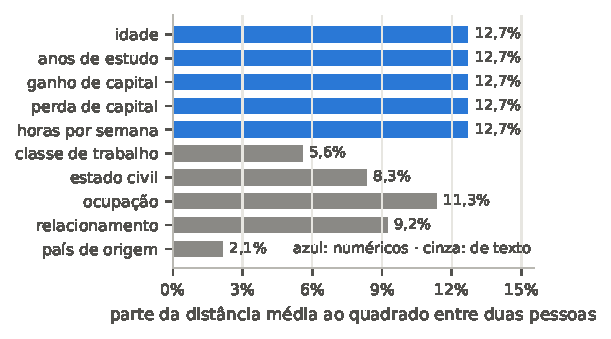
\includegraphics[width=.62\textwidth]{figures/clusters_peso.pdf}
\caption{Parte de cada atributo na distância média ao quadrado entre duas pessoas sorteadas (\clColunas{} colunas, com log no capital).}
\label{fig:cl_peso}
\end{figure}

\subsection{O efeito do logaritmo no capital}\label{sec:cl_log}

O ganho e a perda de capital são zero para quase todos: só \clComGanho\% das pessoas têm algum ganho e \clComPerda\% alguma perda, e poucos valores são muito altos. Padronizado sem log, o ganho de 99.999 dólares, o teto do censo, fica a \clSemLogMax{} desvios da média, e as \clTeto{} pessoas com esse valor formam um grupo só delas (Tabela~\ref{tab:cl_log}). Com o log, o máximo cai para \clComLogMax{} desvios e esse grupo desaparece. Surge, porém, outro efeito: quem não tem ganho fica em \clComLogZero{} desvio, e quem tem algum ganho fica perto de $+3$, um salto maior que qualquer troca de categoria. As \clComLogGanho{} pessoas com ganho e as \clComLogPerda{} com perda formam grupos próprios, com \clComLogGanhoPos\% e \clComLogPerdaPos\% acima de 50 mil. Mantivemos o log: esses dois grupos são reais e concentram a renda alta, enquanto o grupo das \clTeto{} pessoas é um artefato do teto do censo. A consequência é que, de $k = 4$ em diante, dois dos $k$ grupos ficam com os \clComCapital\% das pessoas que têm capital, e os demais dividem o resto.

\begin{table}[ht]
\centering
\caption{K-means com $k = 4$ e seed 42, sem e com log no ganho e na perda de capital.}
\label{tab:cl_log}
\footnotesize
\begin{tabular}{lrrrr}
\toprule
Grupo (k = 4, seed 42) & Pessoas & Com ganho (\%) & Com perda (\%) & $>$50K (\%) \\
\midrule
\multicolumn{5}{l}{\emph{Sem log}} \\
1º maior & 16.888 & 11,3 & 0,1 & 36,7 \\
2º maior & 11.709 & 4,1 & 0,1 & 3,7 \\
3º maior & 1.394 & 0,0 & 100,0 & 52,7 \\
4º maior & 148 & 100,0 & 0,0 & 100,0 \\
\midrule
\multicolumn{5}{l}{\emph{Com log}} \\
1º maior & 15.496 & 0,0 & 0,0 & 31,6 \\
2º maior & 10.706 & 0,3 & 0,0 & 2,6 \\
3º maior & 2.510 & 100,0 & 0,0 & 63,5 \\
4º maior & 1.427 & 0,0 & 100,0 & 51,6 \\
\bottomrule
\end{tabular}

\end{table}

A Figura~\ref{fig:cl_log} estende a comparação a todo $k$ de 2 a 10, na seed 42. Sem log, o menor grupo tem sempre \clSemLogMenor{} pessoas de $k = 4$ em diante: o grupo do teto do censo aparece em qualquer partição com quatro grupos ou mais, e a silhueta fica abaixo da versão com log (\clSemLogSilSeis{} contra \clComLogSilSeis{} em $k = 6$). A exceção é $k = 2$, em que a versão sem log tem silhueta maior (\clSemLogSilDois), porque separa só as \clSemLogMenorDois{} pessoas com perda de capital. Com log, o menor grupo passa a ser o das \clComLogMenor{} pessoas com perda, de $k = 3$ em diante: o logaritmo troca um grupo artificial por um grupo real.

\begin{figure}[ht]
\centering
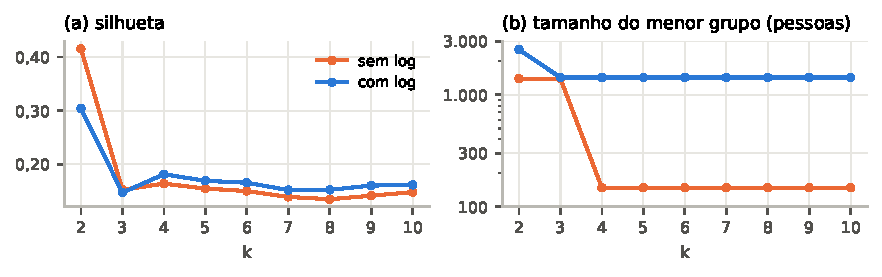
\includegraphics[width=\textwidth]{figures/clusters_log.pdf}
\caption{K-means sem e com log no capital, para $k$ de 2 a 10 (seed 42): silhueta e tamanho do menor grupo (escala logarítmica).}
\label{fig:cl_log}
\end{figure}

\subsection{Escolha do número de grupos}\label{sec:cl_k}

As métricas internas não apontam um $k$ claro (Figura~\ref{fig:cl_curvas} e Tabela~\ref{tab:cl_k}). Silhueta e Davies-Bouldin preferem $k = 2$ (\clSilDois{} e \clDbDois), mas esse $k$ só separa quem tem ganho de capital do resto: é a fronteira mais nítida da base, e diz pouco sobre as demais pessoas. Em 9 seeds o grupo pequeno é o do ganho; numa, o da perda, com quase a mesma inércia, o que explica o ARI mínimo de \clAriDoisMin{} entre seeds. De $k = 4$ em diante, as duas métricas ficam planas, com silhueta em torno de \clSilSeis. Valores tão baixos (acima de 0,5 indicariam grupos bem separados) mostram que a base não tem grupos nítidos: os grupos são regiões de uma nuvem contínua de pessoas. Na inércia, a queda de um $k$ para o seguinte passa de \clQuedaQuatroCinco{} (de 4 para 5) para \clQuedaCincoSeis{} (de 5 para 6) e \clQuedaSeisSete{} (de 6 para 7): o cotovelo fica entre 5 e 6.

\begin{figure}[ht]
\centering
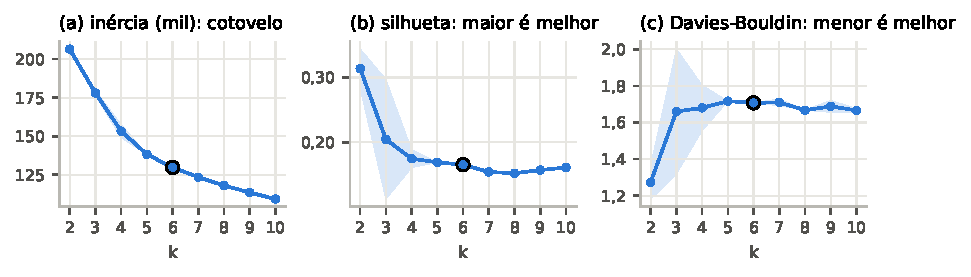
\includegraphics[width=\textwidth]{figures/clusters_curvas.pdf}
\caption{Métricas internas para $k$ de 2 a 10: média das 10 seeds (linha) e $\pm$ um desvio (faixa); o círculo marca $k = 6$.}
\label{fig:cl_curvas}
\end{figure}

\begin{table}[ht]
\centering
\caption{Métricas internas (média das 10 seeds) e estabilidade (ARI médio entre as seeds, 45 pares) por $k$.}
\label{tab:cl_k}
\footnotesize
\begin{tabular}{crrrrr}
\toprule
k & Inércia & Silhueta & Davies-Bouldin & ARI (10 inic.) & ARI (1 inic.) \\
\midrule
2 & 206.442 & 0,314 & 1,27 & 0,789 & 0,786 \\
3 & 178.031 & 0,204 & 1,66 & 0,589 & 0,605 \\
4 & 153.330 & 0,175 & 1,68 & 0,858 & 0,717 \\
5 & 138.247 & 0,169 & 1,72 & 0,977 & 0,856 \\
\textbf{6} & 129.755 & 0,165 & 1,71 & 0,995 & 0,588 \\
7 & 123.438 & 0,154 & 1,71 & 0,926 & 0,558 \\
8 & 118.019 & 0,152 & 1,67 & 0,997 & 0,566 \\
9 & 113.503 & 0,157 & 1,69 & 0,786 & 0,649 \\
10 & 109.249 & 0,161 & 1,67 & 0,904 & 0,730 \\
\bottomrule
\end{tabular}

\end{table}

Como as métricas empatam, a estabilidade desempata (Figura~\ref{fig:cl_estab}). Com 10 inicializações, as 10 seeds chegam praticamente à mesma partição em $k = 5$, 6 e 8 (ARI de \clAriCinco, \clAriSeis{} e \clAriOito), enquanto $k = 3$ (\clAriTres) e $k = 9$ (\clAriNove) são instáveis: o algoritmo corta uma região sem fronteira natural, e cada seed corta de um jeito. Com uma só inicialização por seed, cada sorteio para num mínimo local diferente: em $k = 6$, o ARI cai para \clAriSeisUm, e a inércia média piora entre \clPioraMin\% e \clPioraMax\% conforme o $k$. As 10 inicializações custam 10 vezes mais e compram a mesma resposta em todas as seeds.

\begin{figure}[ht]
\centering
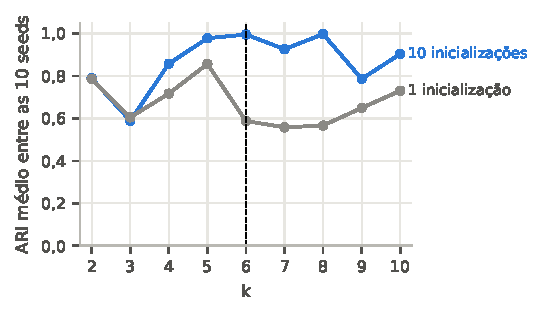
\includegraphics[width=.62\textwidth]{figures/clusters_estabilidade.pdf}
\caption{Estabilidade: ARI médio entre as partições das 10 seeds, com 10 inicializações por seed e com uma só.}
\label{fig:cl_estab}
\end{figure}

Escolhemos $k = 6$: está no cotovelo, é praticamente estável (ARI de \clAriSeis) e, como dois grupos ficam com o capital, deixa quatro grupos para quem não o tem. A Tabela~\ref{tab:cl_alt} mostra os dois vizinhos estáveis, $k = 5$ e $k = 8$, na seed 42. Os dois grupos do capital são os mesmos nos três $k$. Com $k = 5$, sobram três grupos sem capital: jovens solteiros, casados com pouco estudo e casados com muito estudo; os mais velhos sem cônjuge ficam diluídos entre os outros. Com $k = 8$, os jovens se dividem pelas horas de trabalho (22 anos e 20 horas por semana; 28 anos e 41 horas), surge um grupo de quem trabalha 66 horas por semana, e os mais velhos sem cônjuge continuam num grupo próprio, agora com 55 anos em média. O $k = 6$ é o menor $k$ que separa os mais velhos sem cônjuge dos casados, sem dividir os jovens por detalhes. A escolha combina métricas e interpretação, e $k = 5$ ou $k = 8$ também seriam defensáveis.

\begin{table}[ht]
\centering
\caption{As alternativas estáveis: perfis com $k = 5$ e $k = 8$ (seed 42), com os grupos ordenados pelo \% acima de 50 mil.}
\label{tab:cl_alt}
\scriptsize
\setlength{\tabcolsep}{3pt}
\begin{tabular}{clrrrrrlr}
\toprule
k & Grupo & Pessoas & Idade & \shortstack{Anos de\\estudo} & \shortstack{Horas por\\semana} & \shortstack{Casados\\(\%)} & Ocupação mais comum & \shortstack{$>$50K\\(\%)} \\
\midrule
5 & 1 & 9.282 & 25,9 & 9,6 & 34,9 & 7 & outros serviços & 1,8 \\
 & 2 & 9.313 & 47,6 & 8,5 & 38,9 & 61 & ofícios e reparos & 18,7 \\
 & 3 & 7.608 & 40,2 & 12,3 & 49,3 & 66 & especialista & 42,9 \\
 & 4 (todos com perda) & 1.427 & 41,6 & 11,0 & 43,5 & 64 & gerência & 51,6 \\
 & 5 (todos com ganho) & 2.509 & 43,8 & 11,1 & 44,2 & 68 & especialista & 63,6 \\
\midrule
8 & 1 & 2.551 & 22,9 & 9,2 & 20,3 & 6 & outros serviços & 1,1 \\
 & 2 & 7.403 & 28,5 & 9,8 & 41,1 & 1 & administrativo & 2,3 \\
 & 3 & 4.479 & 55,2 & 8,2 & 36,4 & 37 & administrativo & 11,6 \\
 & 4 & 5.344 & 37,5 & 9,0 & 41,9 & 100 & ofícios e reparos & 28,7 \\
 & 5 & 1.881 & 40,4 & 10,3 & 66,3 & 66 & gerência & 33,5 \\
 & 6 & 4.570 & 43,2 & 13,4 & 42,4 & 66 & especialista & 50,2 \\
 & 7 (todos com perda) & 1.427 & 41,6 & 11,0 & 43,5 & 64 & gerência & 51,6 \\
 & 8 (todos com ganho) & 2.484 & 43,7 & 11,2 & 44,2 & 68 & especialista & 64,1 \\
\bottomrule
\end{tabular}

\end{table}

\subsection{Os seis grupos}\label{sec:cl_grupos}

A partição da seed 42 coincide com as das seeds 0 a 9 (ARI entre 0,977 e 0,999 com cada uma). A Tabela~\ref{tab:cl_grupos} resume os grupos; os nomes são nossos, tirados do perfil médio, e o K-means devolve só um número por pessoa. Os grupos 1 a 4, sem capital, se separam pela fase da vida e pelo tipo de trabalho: jovens que nunca se casaram e muitas vezes moram com os pais (grupo 1); pessoas mais velhas, divorciadas ou viúvas, com pouco estudo (grupo 2); casados em ofícios manuais, com jornadas longas (grupo 3); e profissionais com muito estudo, especialistas e gerentes (grupo 4). Os grupos 5 e 6 são parecidos entre si nos demais atributos (cerca de 42 anos, 11 anos de estudo, dois terços casados): o que os separa do resto, e um do outro, é o capital.

\begin{table}[ht]
\centering
\caption{Perfil dos seis grupos ($k = 6$, seed 42): médias dos numéricos, \% de casados, a ocupação mais comum (com a sua parte no grupo) e \% acima de 50 mil.}
\label{tab:cl_grupos}
\scriptsize
\setlength{\tabcolsep}{3pt}
\begin{tabular}{lrrrrrlr}
\toprule
Grupo & Pessoas & Idade & \shortstack{Anos de\\estudo} & \shortstack{Horas por\\semana} & \shortstack{Casados\\(\%)} & Ocupação mais comum & \shortstack{$>$50K\\(\%)} \\
\midrule
1. Jovens solteiros & 8.439 & 25,7 & 9,4 & 34,4 & 3 & outros serviços (20\%) & 1,1 \\
2. Mais velhos sem cônjuge & 5.443 & 53,4 & 8,5 & 36,3 & 37 & administrativo (18\%) & 12,6 \\
3. Casados em ofícios manuais & 6.538 & 37,6 & 9,0 & 47,6 & 90 & ofícios e reparos (26\%) & 27,5 \\
4. Profissionais com muito estudo & 5.791 & 40,9 & 13,3 & 45,1 & 57 & especialista (40\%) & 44,8 \\
5. Com perda de capital & 1.427 & 41,6 & 11,0 & 43,5 & 64 & gerência (20\%) & 51,6 \\
6. Com ganho de capital & 2.501 & 43,7 & 11,2 & 44,3 & 68 & especialista (22\%) & 63,8 \\
\midrule
Base inteira & 30.139 & 38,4 & 10,1 & 40,9 & 47 & especialista (13\%) & 24,9 \\
\bottomrule
\end{tabular}

\end{table}

A categoria mais comum resume pouco: a Figura~\ref{fig:cl_prop} mostra a composição de cada grupo em estado civil, relacionamento e ocupação. O grupo 1 tem \clNuncaUm\% de pessoas que nunca se casaram e \clFilhoUm\% de filhos que moram na casa dos pais. O grupo 2 reúne divorciados (\clDivorcDois\%), viúvos (\clViuvoDois\%) e quem chefia a casa sem cônjuge (\clChefeDois\%). O grupo 3 é quase todo de casados (\clCasadosTres\%), e \clMaridoTres\% são maridos, em ofícios, transporte e operação de máquinas. O grupo 4 concentra especialistas (\clEspecQuatro\%) e gerentes (\clGerenQuatro\%). Nos grupos 5 e 6, a composição é parecida com a do grupo 4, com mais casados: o que os separa é o capital, e não o perfil.

\begin{figure}[ht]
\centering
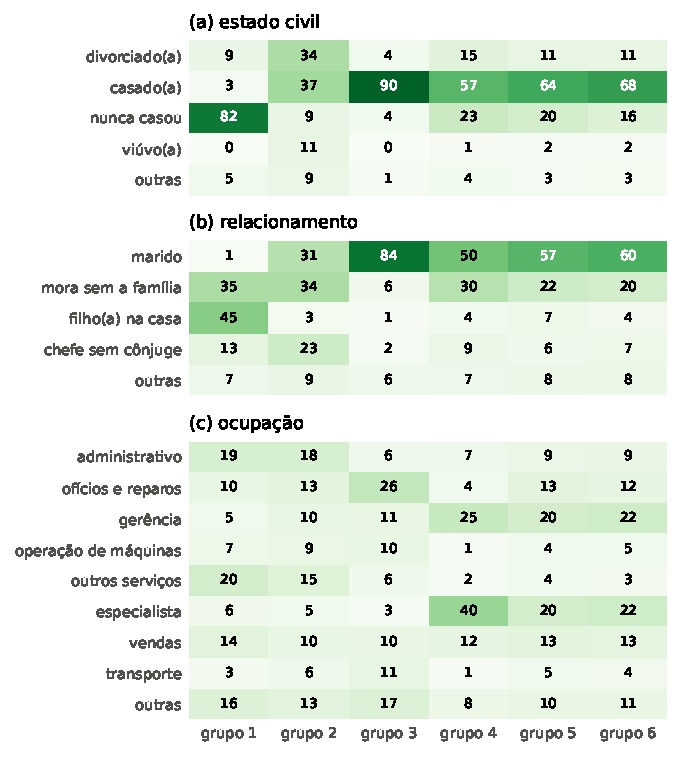
\includegraphics[width=.8\textwidth]{figures/clusters_proporcoes.pdf}
\caption{Composição dos grupos ($k = 6$, seed 42), em \% das pessoas de cada grupo: categorias com pelo menos 10\% em algum grupo; as demais somadas em ``outras''.}
\label{fig:cl_prop}
\end{figure}

A silhueta média, \clSilSeis, esconde diferenças grandes entre os grupos (Figura~\ref{fig:cl_sil}). Os grupos do capital são os mais bem definidos, com silhueta média de \clSilGCinco{} (perda) e \clSilGSeis{} (ganho) e quase nenhuma pessoa com silhueta negativa. Entre os grupos sem capital, os jovens solteiros (\clSilGUm) e os casados em ofícios manuais (\clSilGTres) são os mais coesos, e os profissionais (\clSilGQuatro) já têm \clSilNegGQuatro\% de pessoas mais perto de outro grupo que do próprio. O grupo 2 é o mais difuso: silhueta média de \clSilGDois, com \clSilNegGDois\% das pessoas do lado negativo. Ele reúne quem não se encaixa nos perfis mais nítidos, e é por isso que só aparece a partir de $k = 6$.

\begin{figure}[ht]
\centering
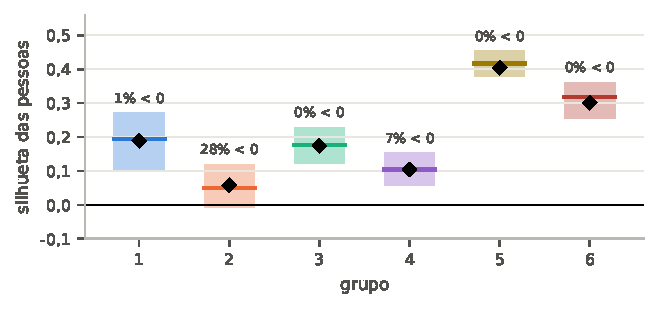
\includegraphics[width=.75\textwidth]{figures/clusters_silhueta.pdf}
\caption{Silhueta das pessoas de cada grupo, na amostra fixa de 10 mil pessoas: a caixa vai do 1º ao 3º quartil, a linha é a mediana, o losango é a média, e o rótulo dá o \% de silhuetas negativas.}
\label{fig:cl_sil}
\end{figure}

A Figura~\ref{fig:cl_pca} projeta as \clColunas{} colunas nas duas direções de maior variância (PCA). A projeção explica só \clVarTotal\% da variância e serve apenas para desenhar, porque o K-means agrupou nas \clColunas{} colunas. Mesmo assim, ela mostra o que as métricas indicaram: os grupos do capital ficam isolados, um em cima e outro embaixo, e os grupos 1 a 4 se encostam numa nuvem contínua, dos jovens solteiros, à esquerda, aos profissionais, à direita.

\begin{figure}[ht]
\centering
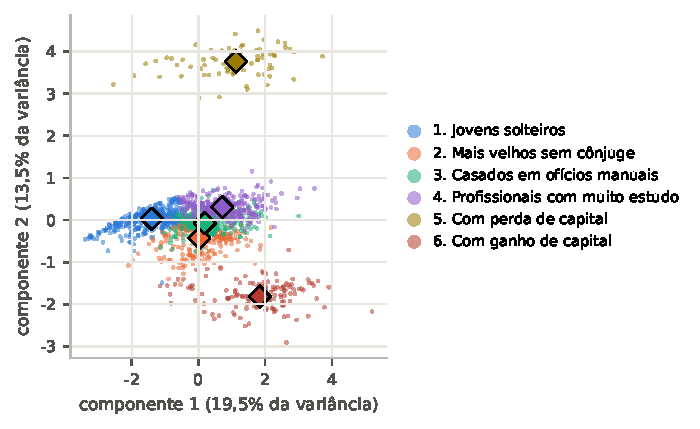
\includegraphics[width=.85\textwidth]{figures/clusters_pca.pdf}
\caption{Os seis grupos nas duas primeiras componentes principais (amostra de 1.500 pessoas); os losangos são os centros dos grupos, calculados com todas as pessoas.}
\label{fig:cl_pca}
\end{figure}

\subsection{Comparação com a renda}\label{sec:cl_renda}

O K-means não viu a renda, e mesmo assim os grupos se ordenam por ela (Figura~\ref{fig:cl_renda}): \clPosUm\% dos jovens solteiros ganham mais de 50 mil, contra \clPosQuatro\% dos profissionais com muito estudo e \clPosSeis\% de quem tem ganho de capital (\clPositivos\% na base inteira). Os atributos que formam os grupos, como idade, estudo, estado civil, ocupação e capital, são os mesmos que explicam a renda.

\begin{figure}[ht]
\centering
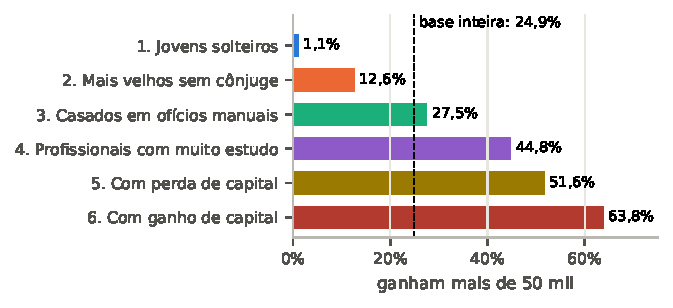
\includegraphics[width=.75\textwidth]{figures/clusters_renda.pdf}
\caption{Percentual de pessoas acima de 50 mil em cada grupo ($k = 6$, seed 42).}
\label{fig:cl_renda}
\end{figure}

Como previsão, porém, os grupos são fracos. Se cada grupo respondesse a renda da sua maioria (os grupos 1 a 4, ``até 50 mil''; os grupos 5 e 6, ``acima''), acertaria \clPureza\% das pessoas, a \emph{pureza} da partição. Responder ``até 50 mil'' para todos já acerta \clChute\%, só \clPurezaGanho{} pontos a menos, e a SVM com kernel RBF, treinada com a renda na parte anterior do trabalho, acerta \clSvmAcc\% no teste (média de 10 divisões). Nenhum grupo é puro: no grupo 4, a chance de renda alta é de \clPosQuatro\%, quase a de uma moeda. O ARI entre os grupos e as duas classes de renda é de \clAriRenda, perto do acaso; com seis grupos e duas classes, ele não chegaria a 1 nem com grupos puros, e por isso a pureza é a métrica mais fácil de ler. O K-means junta pessoas parecidas em todos os atributos, com o mesmo peso para os que importam muito e os que importam pouco para a renda; um classificador aprende com a renda onde fica a fronteira. Os grupos servem para descrever a população, e não para prever a renda de uma pessoa.

\subsection{Raça e sexo nos grupos}\label{sec:cl_sensiveis}

Raça e sexo ficaram fora do agrupamento, como ficaram fora da classificação na parte anterior do trabalho, porque não queremos que o perfil de uma pessoa seja definido por eles. Usamos os dois só depois, para ver como se distribuem nos grupos formados pelos outros atributos (Tabela~\ref{tab:cl_sensiveis}). Por decisão do grupo, essa análise aparece só neste relatório e não nos slides: em uma apresentação curta, os números ficariam sem o contexto que os explica e poderiam ser lidos como uma afirmação sobre pessoas, quando dizem respeito à forma como a base e os atributos foram construídos.

\begin{table}[ht]
\centering
\caption{Sexo e raça em cada grupo ($k = 6$, seed 42), em \% das pessoas do grupo. Nenhum dos dois entrou no agrupamento.}
\label{tab:cl_sensiveis}
\footnotesize
\begin{tabular}{lrrrrrrr}
\toprule
(\%) & Grupo 1 & Grupo 2 & Grupo 3 & Grupo 4 & Grupo 5 & Grupo 6 & Base \\
\midrule
Mulheres & 47,7 & 48,3 & 8,3 & 29,2 & 23,6 & 21,8 & 32,4 \\
\midrule
\multicolumn{8}{l}{\emph{Raça}} \\
Branca & 81,9 & 82,7 & 89,5 & 88,6 & 89,8 & 89,4 & 86,0 \\
Negra & 12,8 & 13,4 & 6,6 & 5,7 & 6,2 & 6,4 & 9,3 \\
Asiática ou do Pacífico & 3,1 & 2,3 & 1,9 & 4,7 & 3,1 & 2,8 & 3,0 \\
Indígena ou esquimó & 1,1 & 1,0 & 1,1 & 0,5 & 0,4 & 0,9 & 0,9 \\
Outra & 1,1 & 0,6 & 0,9 & 0,5 & 0,5 & 0,4 & 0,8 \\
\bottomrule
\end{tabular}

\end{table}

Mesmo fora do agrupamento, os dois se distribuem de forma desigual. O grupo 3 tem só \clMulheresTres\% de mulheres, porque ``marido'', o relacionamento de 84\% do grupo, indica o sexo quase sem exceção. Os grupos 1 e 2, os de menor renda, têm \clMulheresUm\% e \clMulheresDois\% de mulheres (\clMulheresBase\% na base) e a maior proporção de pessoas negras (\clNegrosUm\% e \clNegrosDois\%, contra \clNegrosBase\% na base). Atributos como estado civil, relacionamento e ocupação carregam essa informação, e os grupos a refletem: tirar raça e sexo da entrada não os tira do resultado.

\subsection{Custo}\label{sec:cl_custo}

Cada iteração do K-means custa proporcionalmente ao número de pessoas, ao número de grupos e ao de colunas, e o custo total cresce linearmente com a base. Um ajuste com $k = 6$ e 10 inicializações leva \clTempoSeis{} s nas \clLinhas{} pessoas, num núcleo (\clTempoSeisUm{} s com uma inicialização), e o estudo inteiro, com \clAjustes{} ajustes, cerca de 4 minutos. A Figura~\ref{fig:cl_tempo} mostra o tempo por $k$: ele cresce de \clTempoDois{} s em $k = 2$ para cerca de 1 s de $k = 5$ em diante, acompanhando o número de iterações até a partição parar de mudar (de \clIterDois{} em $k = 2$ para \clIterSeis{} em $k = 6$ e \clIterDez{} em $k = 10$). Com mais grupos, há mais fronteiras a ajustar, e os centros levam mais passos para se acomodar. Com uma só inicialização, o custo cai para cerca de um décimo, mas a resposta muda de uma seed para outra (Seção~\ref{sec:cl_k}).

\begin{figure}[ht]
\centering
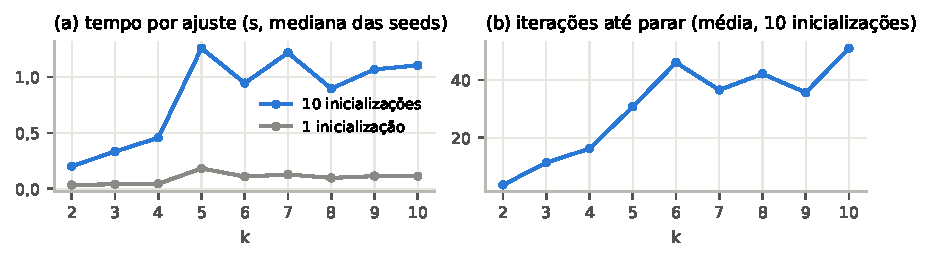
\includegraphics[width=\textwidth]{figures/clusters_tempo.pdf}
\caption{Custo do K-means por $k$, num único núcleo, nas \clLinhas{} pessoas: tempo por ajuste (mediana das 10 seeds) e número médio de iterações.}
\label{fig:cl_tempo}
\end{figure}
